\documentclass[a4paper]{article}
%
% importar el archivo conf/packages.tex
%
% ===
% === Trick para detectar si el documento está siendo compilado con pdflatex
% ===
%
% Esto me setea la variable pdf dependiendo del valor de \pdfoutput, que es >0
% sólo cuando estoy usando pdflatex para compilar el documento. Con esto puedo
% hacer  \ifpdf {...} \fi, que se ejecuta colo cuando compilo con pdflatex.
\newif\ifpdf
\ifnum\pdfoutput<0
\pdffalse\fi
\ifnum\pdfoutput=0
\pdffalse\fi
\ifnum\pdfoutput>0
\pdftrue\fi
%
% ===
% === I18n / L10n
% ===
%
% babel me da separación de sílabas para palabras en el idioma que le paso como
%       argumento opcional.
\usepackage[spanish]{babel}
%
% inputenc define la codificación de caracteres del código fuente, acá utf8.
\usepackage[utf8]{inputenc}
%
% ===
% === Gráficos
% ===
% 
% pst-pdf me permite usar PSTricks con pdflatex. Necesito cargarlo sólo si está
%         definida la variable pdf, por eso está entre \ifpdf ... \fi
\ifpdf\usepackage{pst-pdf}\fi
%
% color me permite usar colores en el documento.
\usepackage{color}
%
% graphicx me da el comando \includegraphics para insertar imágenes (?)
\usepackage{graphicx}
%
% pstricks es un conjunto de macros basadas en PostScript para TeX, en
%          castellano: me da un entorno pstricks y comandos que uso dentro de
%          éste, que me sirven para dibujar figuras/diagramas/etc de manera
%          relativamente simple.
\usepackage{pstricks}
%
% pst-circ me da macros para pstricks que me dibujan elementos de circuitos
%\usepackage{pst-circ}
%
% pst-plot me provee de funciones de ploteo para pstricks
%\usepackage{pst-plot}
%
% pst-2dplot me sirve para plotear en pstricks, entorno pstaxes
%\usepackage{pst-2dplot}
%
% ===
% === Verbatims
% ===
%
% verbatim es una reimplementación de los entornos verbatim[*]
%          provee el comando \verbatiminput{archivo} y el entorno comment, que
%          hace que LaTeX ignore directamente todo lo que está adentro
\usepackage{verbatim}
%
% moreverb implementa el entorno verbatimtab indentando los tabs que encuentre,
%          y también el entorno listing, que pone números de línea al verbatim.
%          Para cambiar el ancho de la tabulacion, uso
%          \renewcommand\verbatimtabsize{<ancho del tab>\relax}
%          También define el entorno boxedverbatim.
\usepackage{moreverb}
%
% listings me da el entorno lstlisting con resaltado de sintaxis.
%          Para setear el lenguaje del código, hago \lstset{language=<lang>}
\usepackage{listings}
%
% url es un verbatim para escribir URL's que permite linebreaks dentro de ésta.
%     para usarlo, \url{<URL>}
\usepackage{url}
%
% ===
% === Más packages
% ===
%
\usepackage{mdwlist}		%Para listas mas compactas
\usepackage{textcomp}		%Para algunos símbolos
\usepackage{colortbl}		%Para celdas de colores en tablas
\usepackage{fancyhdr}		%Para encabezados/pie
\usepackage{bbold}		%Fuente bb para modo math: \mathbb{R} = reales
\usepackage{dsfont}		%Fuente ds para modo math: \mathds{R} = reales
\usepackage{multirow}		%Para "combinar" celdas en tablas
\usepackage{float}		%Para cuadros, figuras, etc copadas
\usepackage{fancybox}		%Para recuardos de texto con bordes "fancy"
\usepackage{dingbat}		%Para dingbats
%\usepackage{marginal}		%Para notas al margen que no puedo hacer andar
\usepackage{amsmath}		%Para enornos matemáticos mas flexibles
%\usepackage{varwidth}		%varwidth es un minipage que se ajusta al ancho mínimo

%
% ===
% === Propiedades del documento: título, autor, etc
% ===
%
\newcommand{\titulo}{{\large FICH --- UNL}\\Redes y Comunicaciones de datos 2 -- 2010\\TP N° 1}
\newcommand{\autor}{Fornal, Esteban \and Mastaglia, Nicolás \and Pfarher, Christian \and Torrez, Mauro}
\newcommand{\fecha}{\today}
\newcommand{\tituloPDF}{Redes 2 1010 - TP1}
\newcommand{\autorPDF}{Fornal -- Mastaglis -- Pfarher -- Torrez}
\newcommand{\asuntoPDF}{TP 1 de Redes 2 2010}
\newcommand{\clavesPDF}{redes tp 1}
%
% importar los archivos conf/config.tex y conf/comandos.tex
% config.tex: configuraciones del documento
\selectlanguage{spanish}		%Elijo idioma español

%Permitir que los entornos equation, align, etc permitan saltos de página
\allowdisplaybreaks[1]

%Tweaks
\setlength{\parindent}{0mm}		%Sangría de 1a. línea
\setlength{\hoffset}{-5.4mm}		%
\setlength{\voffset}{-5.4mm}		%
\setlength{\topmargin}{0mm}		%
\setlength{\oddsidemargin}{5mm}	%
\setlength{\evensidemargin}{5mm}	%
\setlength{\marginparsep}{5mm}	%
\setlength{\headheight}{12.5mm}	%
\setlength{\headsep}{2.5mm}		%
\setlength{\footskip}{10mm}		%
\setlength{\textwidth}{15cm}		%
\setlength{\textheight}{232mm}	%
\setlength{\fboxrule}{.1pt}
\setlength{\parskip}{.5\baselineskip}

%Colores
\definecolor{negro}	{cmyk}{0,0,0,1}
\definecolor{marron}	{cmyk}{0,.5,1,.41}
\definecolor{rojo}	{cmyk}{0,1,1,0}
\definecolor{naranja}	{cmyk}{0,.35,1,0}
\definecolor{amarillo}	{cmyk}{0,0,1,0}
\definecolor{verde}	{cmyk}{1,0,1,0}
\definecolor{azul}	{cmyk}{1,1,0,0}
\definecolor{violeta}	{cmyk}{.45,1,0,0}
\definecolor{gris}	{cmyk}{0,0,0,.5}
\definecolor{blanco}	{cmyk}{0,0,0,0}
\definecolor{dorado}	{cmyk}{0,.16,1,0}
\definecolor{plateado}	{cmyk}{0,0,0,.25}

\title{\titulo}
\author{\autor}
\date{\fecha}

% si uso pdflatex, me setea las propiedades del pdf de salida
\ifpdf\pdfinfo{/Title    (\tituloPDF)
               /Author   (\autorPDF)
               /Subject  (\asuntoPDF)
               /Keywords (\clavesPDF)}\fi




% comandos.tex
% en este archivo defino todos los comandos/environment que quiera usar en mi documento.
%
% ===
% === Comandos
% ===
% 
% T: para escribir texto común cuando en modo math
%    uso: \T{texto que aparecerá en letra normal}
\newcommand{\T}{\textrm}
%
% aclaracion: dibuja un recuadrito aclaratorio, como <quote> en HTML.
%             uso: \aclaracion{Texto...}
\newcommand{\aclaracion}[1]{%
\smallpencil\ \begin{minipage}{0.9\textwidth}
\vspace*{6pt}{#1}\smallskip\end{minipage}}
%
% consigna: parecido a aclaración, pero con texto _slanted_
%           uso: \consigna{Consigna...}
\newcommand{\consigna}[1]{%
\leftpointright\ \parbox[t]{0.9\textwidth}{\textsl{#1}\vspace{8pt}}}
%
% pinterno: para representar el producto interno entre los dos argumentos
%           uso: \pinterno{X}{Y}
\newcommand{\pinterno}[2]{%
\left\langle #1 , #2 \right\rangle}
%
% === Estilos de texto
%
% resalt: resaltado con fondo verde
%         uso: \resalt{texto resaltado}
\newcommand{\resalt}{\colorbox{green}}
%
% sfbf: texto en negrita + slanted
%       uso: 
\newcommand{\sfbf}{\bfseries\textsf}
%
% eng: itálica (para palabras en inglés)
%      uso: \eng{some English text}
\newcommand{\eng}{\textit}
%
% mean: significado de una sigla - slanted
%       uso: (...) SNCF: \mean{Société Nationale des Chemins de Fer Francais} ...
\newcommand{\mean}{\textsl}
%
% defin: pone en negrita el texto, útil para definiciones
%        uso: \defin{asshole}: vulgar slang for anus
\newcommand{\defin}{\textbf}
%
% R, N: cambia la tipografía en modo math, probar para ver cómo quedan
%       uso: \R{R} , \N{N}
\newcommand{\R}{\mathds}
\newcommand{\N}{\mathbf}
%
% lil: para escribir texto pequeño. más cómodo que { \footnotesize texto pequeño... }
%      uso: \lil{texto pequeño... }
\newcommand{\lil}[1]{\footnotesize #1}  %Para texto pequeñooo
%
% mono: escribe el texto que le paso como parámetro con letra de ancho fijo
%       uso: \mono{texto monoespaciado}
\newcommand{\mono}[1]{{\tt #1}}
%
% === Símbolos
%
\newcommand{\y}{\wedge}			%Y (Lógica)
\newcommand{\ve}{\vee}			%O (Lógica)
\newcommand{\ent}{\supset}		%Entonces (Lógica)
\newcommand{\dimp}{\leftrightarrow}	%Doble implicativo, equivalencia (Lógica)
\newcommand{\sii}{\leftrightarrow}	%Si y sólo si (Lógica)
\newcommand{\equi}{\equiv}		%Equivalencia (Lógica)
\newcommand{\portanto}{\vdash}		%Por lo tanto (Lógica)
\newcommand{\por}{\cdot}		%Producto punto
\newcommand{\RR}[1][1]{\mathds{R}}	%R de reales
%
%
% ===
% === Environments
% ===
% 
% enunciado: un environment que básicamente tiene el mismo efecto que el
%            comando consigna.
%            uso: \begin{enunciado} ... contenido ... \end{enunciado}
\newenvironment{enunciado}
{\leftpointright\ \begin{varwidth}[t]{0.9\textwidth}\textsl}
{\end{varwidth}\vspace{8pt}}
%
% pvi: para tipear la definición de un problema de valor inicial/funciones
%      definidas de a trozos/etc directamente en el texto (sin necesidad de
%      cambiar a un modo matemático.
%      uso: \begin{pvi} linea1 \\ linea 2 \\ ... \end{pvi}
\newenvironment{pvi}{\begin{equation*}\begin{cases}}
{\end{cases}\end{equation*}}
%
% verbatimsmall: un verbatim con letra más chica. usualmente queda bastante
%                mejor que el verbatim pelado.
%                uso: \begin{verbatimsmall} ........ \end{verbatimsmall}
\newenvironment{verbatimsmall}{\small\begin{verbatim*}}
{\end{verbatim*}}
%
%
% ===
% === Comandos ``históricos''
% ===
%
%% %\begin{pspicture}
%% \def\tierra(#1){%Para dibujar el símbolo de tierra en el entorno PSTricks
%% 	\rput(#1){
%% 		\psdot(0,0)
%% 		\psline(0,0)(0,-0.45)
%% 		\psline(-0.5,-0.45)(0.5,-0.45)
%% 		\psline(-0.35,-0.6)(0.35,-0.6)
%% 		\psline(-0.2,-0.75)(0.2,-0.75)
%% 	}%
%% }
%% %\end{pspicture}

%% \newcommand{\codigo}[2]{%Para generar un recuadro con código
%% 	%\setlength{\hrulewidth}{0.1pt}
%% 	\begin{flushleft}
%% 	\underline{#1}
%% 	\begin{tabular}{@{\quad}|l}
%% 		\begin{minipage}{.85\textwidth}\smallskip{#2}
%% 	\end{minipage}\end{tabular}\end{flushleft}%
%% }

%% \newcommand{\filecodigo}[1]{%Insertar código verbatim desde un archivo
%% \codigo{#1}{\verbatiminput{#1}}}%Requiere el paquete verbatim
%% \newcommand{\filecodigobis}[1]{{\verbatiminput{#1}}}%Requiere el paquete verbatim

%% \newcommand{\grafico}[3][1]{%Para generar un plot de un archivo con coords.
%% %\def\deequis=#1
%% \begin{minipage}{0.5\textwidth}\begin{center}
%% \begin{pspicture}(6,5)
%% 	\psgrid[subgriddiv=1,gridlabels=0pt,gridwidth=.1pt](1,3)(1,1)(6,5)
%% 	\psset{xunit=5cm,yunit=2cm}
%% 	\fileplot[linewidth=1pt,linecolor=blue,origin={0.2,1.5}]{#2}
%% 	\psset{xunit=1cm,yunit=1cm}
%% 	\psaxes[Dx=#1,dx=5,Oy=-1,Dy=1,dy=2]{-}(0.9,1)(6,5)
%% 	\rput(4,0.4){\textsl{#3}}
%% \end{pspicture}\end{center}\end{minipage}}

%% \newcommand{\eqncode}[2]{%
%% \begin{center}
%% \begin{tabular}{l@{\hspace{0.5cm}}r}
%% \begin{minipage}{.4\textwidth}
%% \begin{equation*}
%% #1
%% \end{equation*}
%% \end{minipage}
%% &
%% \fbox{\begin{minipage}{.4\textwidth}
%% %\setlength{\parskip}{4mm}
%% \filecodigobis{#2}
%% \end{minipage}}
%% \end{tabular}
%% \end{center}
%% }

%% \newcommand{\eqncodeb}[2]{%
%% \begin{center}\begin{tabular}{l@{\hspace{0.5cm}}r}
%% \begin{minipage}{.4\textwidth}#1\end{minipage} &
%% \fbox{\begin{minipage}{.4\textwidth}\filecodigobis{#2}\end{minipage}}
%% \end{tabular}\end{center}}

%% \newenvironment{matemcode}[1]{\newline
%% \begin{tabular}{l@{\hspace{0.5cm}}r}
%% \begin{minipage}{.4\textwidth}
%% \parbox[t]{.4\textwidth}{\begin{equation*}#1\end{equation*}}\end{minipage}
%% &\begin{Sbox}\begin{minipage}{.4\textwidth}}
%% {\end{minipage}\end{Sbox}\fbox{\TheSbox}\end{tabular}\newline}

%% \newenvironment{encuadrar}[1]{\begin{Sbox}\begin{varwidth}{#1\textwidth}}
%% {\end{varwidth}\end{Sbox}\fbox{\TheSbox}}

%% \newenvironment{parboxenv}{\begin{Sbox}}
%% {\end{Sbox}\parbox[t]{.9\textwidth}{\TheSbox}}

%
% ===
% === Inicio del documento
% === 
%
% todo lo que siga a esto hasta \end{document} será ``typeseteado'' por LaTeX/pdfLaTeX
\begin{document}
%
% crear la página de título
\maketitle
%
% 
\section*{Ejercicio de ejemplo 1}
\subsection*{punto a)}
\consigna{Genere el diagrama de polos y ceros...}

Generamos el diagrama con la función \mono{zplane}.
{\small
\begin{verbatim}
  polos=[ 0.95*exp(j*pi/4); 0.95*exp(-j*pi/4); 0.95*exp(j*pi/4); 0.95*exp(-j*pi/4) ];
  ceros=[ 0.80*exp(j*pi/6); 0.80*exp(-j*pi/6); 0.80*exp(j*pi/3); 0.80*exp(-j*pi/3) ];
  zplane( ceros, polos);
\end{verbatim}
}

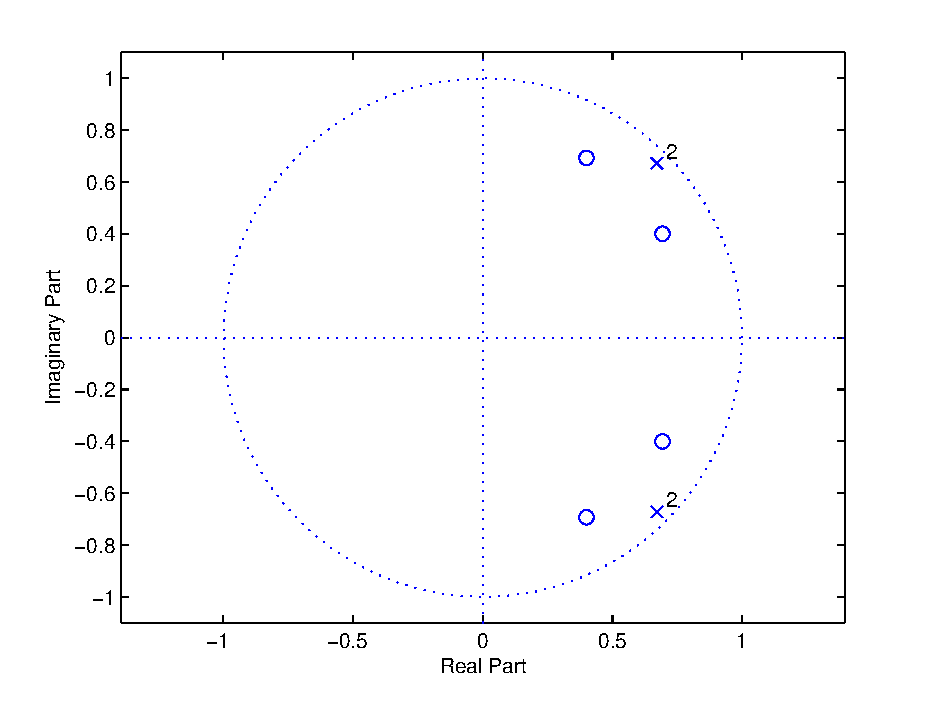
\includegraphics[width=12cm]{img/ej1a}
\newpage
\subsection*{punto f)}

\consigna{...esta vez genere la señal con una frecuencia de muestreo de 120Hz...}

{\small
\verbatiminput{src/ej1f.m}
}
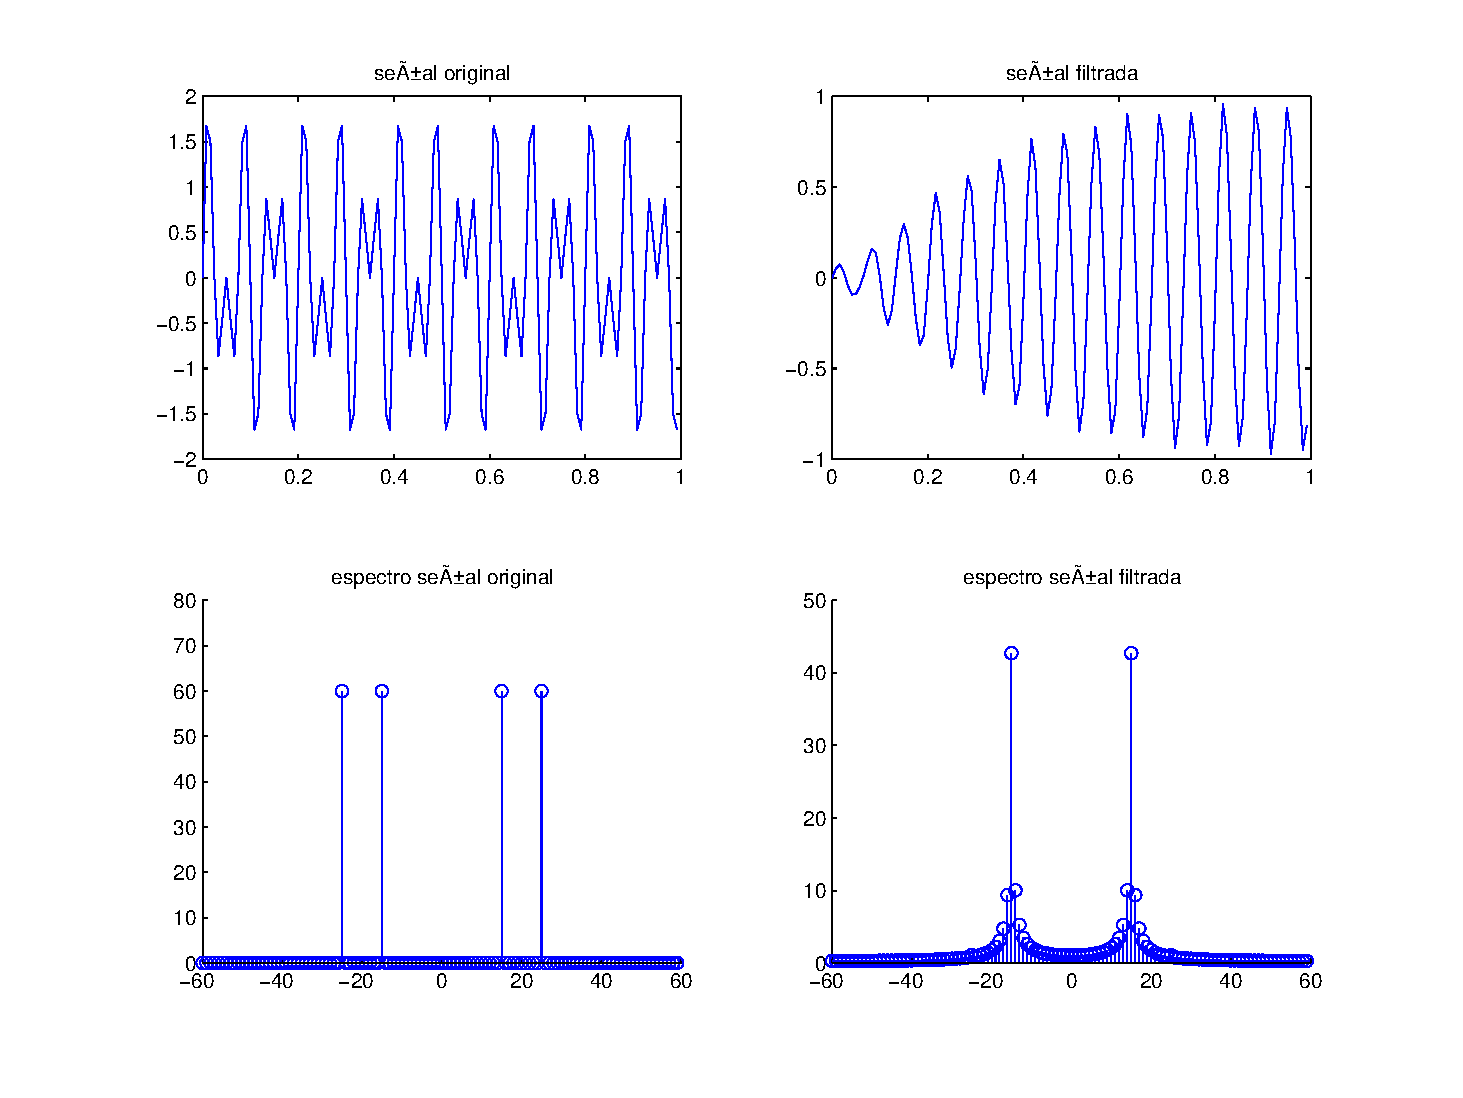
\includegraphics[width=16cm]{img/ej1f}

Vemos que ahora la banda de paso ha quedado centrada en $f=15$Hz
. Esto implica
que el filtro se comportará distinto para distintas frecuencias de muestreo
que utilicemos; en particular, para una frecuencia de muestreo $f_m$ la banda
de paso se centrará en
$$f=\frac{1}{4}\left(\frac{f_m}{2}\right).$$
\newpage
\section*{Ejercicio 2}
%\consigna{Diseñe un filtro pasa-altos de tipo Butterworth con frecuencia de
%corte 500 Hz. Para este ejercicio realice todos los pasos del proceso de diseño,
%comenzando por el diseño analógico y realizando la transformación en frecuencia
%y la transformación conforme. Para obtener el filtro digital correspondiente,
%suponga que se procesarán señales con frecuencia de muestreo 2000 Hz. Utilice
%diferentes órdenes y compare los resultados graficando las respuestas en
%frecuencia.}
La función de transferencia que conocemos para un filtro Butterworth es
\begin{equation*}
\left| H( j\omega ) \right|^2 = \frac{{G_0}^2}{ 1 + \left(
	\frac{\omega}{\omega_c} \right)^{2n} } 
\end{equation*}
donde $n=$ orden del filtro; $\omega_c=$ frecuencia de corte; y $G_0$ es la
componente DC (ganancia en la frecuencia cero).
En términos de $s$, teniendo en cuenta que $s=\sigma+j\omega$, con $\sigma=0$,
podemos ver que:
\begin{equation*}
|H(j\omega)|^2 = \left. H(s)H^*(s)\right|_{s=j\omega}=H(s)H(-s)
= \frac {{G_0}^2}{1+\left (\frac{-s^2}{\omega_c^2}\right)^n}
\end{equation*}
Los polos en esta expresión son los ceros del polinomio de Butterworth $B_n$.
Por ello podemos escribir la función de transferencia en $s$ de un filtro de
Butterworth de la forma
\begin{equation*}
H(s)=\frac{G_0}{B_n}=\frac{G_0}{\prod_{k=1}^n (s-s_k)/\omega_c}\quad\T{donde}
\quad s_k=\omega_c e^{j \frac{2 k +n-1}{2n} \pi}
\end{equation*}
%
\subsection*{Paso 1}
El filtro de Butterworth normalizado ($G_0=1, \omega_c=1$) de grado $n$ viene
dado por:
\begin{equation*}
H(s)=\frac{1}{B_n(s)}=
	\frac{1}{\prod_{k=1}^n\left[s-e^{j\frac{2k+n-1}{2n}\pi}\right]}
\end{equation*}
Los polinomios de Butterworth normalizados de grado 1, 2, 3, 6 son:
\begin{align*}
	B_1(s)&=s-e^{j\frac{2+1-1}{2}\pi}=s-e^{j\pi}=s-(\cos\pi+j\sen\pi)
		=s-(-1+0)\\
		&=s+1\\
	B_2(s)&=\left(s-e^{j\frac{2+2-1}{4}\pi}\right)
		\left(s-e^{j\frac{4+2-1}{4}\pi}\right)
		=\left(s-e^{j\frac{3}{4}\pi}\right)
		\left(s-e^{j\frac{5}{4}\pi}\right)\\
		%&\enspace\vdots\\
		&=\left[s-\left(\cos\frac{3}{4}\pi+j\sen\frac{3}{4}\pi\right)\right]
		\left[s-\left(\cos\frac{5}{4}\pi+j\sen\frac{5}{4}\pi\right)\right]\\
		&=\left[s-\left(-\frac{\sqrt{2}}{2}+j\frac{\sqrt{2}}{2}\right)\right]
\left[s-\left(-\frac{\sqrt{2}}{2}-j\frac{\sqrt{2}}{2}\right)\right]
		=\left[s+\frac{\sqrt{2}}{2}(1-j)\right]
		\left[s+\frac{\sqrt{2}}{2}(1+j)\right]\\
		%&\enspace\vdots\\
		&=s^2+s\sqrt{2}+1\\
	B_3(s)&=\left(s-e^{j\frac{2+3-1}{6}\pi}\right)  \left(s-e^{j
		\frac{4+3-1}{6}\pi}\right)  \left(s-e^{j\frac{6+3-1}{6}\pi}\right)
		=\left(s-e^{j\frac{2}{3}\pi}\right)  \left(s-e^{j
		\pi}\right)  \left(s-e^{j\frac{4}{3}\pi}\right)\\
		&=\left[s-\left(\cos\frac{2}{3}\pi+j\sen\frac{2}{3}\pi\right)\right]
		\left[s-\left(\cos\pi+j\sen\pi\right)\right]
		\left[s-\left(\cos\frac{4}{3}\pi+j\sen\frac{4}{3}\pi\right)\right]\\
		&=\left[s-\left(-\frac{1}{2}+j\frac{\sqrt{3}}{2}\right)\right]
		\left[s-\left(-1\right)\right]
		\left[s-\left(-\frac{1}{2}-j\frac{\sqrt{3}}{2}\right)\right]\\
		&\enspace\vdots\\
		&=\left(s+1\right)\left[s^2+s+1\right]\\
		&=s^3+2s^2+2s+1\\
\end{align*}
\subsection*{Paso 2}
Transformación en frecuencia pasa-bajos $\rightarrow$ pasa-altos:
\begin{equation*}
s\rightarrow\frac{\omega_p}{s}=\frac{2\pi500}{s}
\end{equation*}
Las funciones de transferencia me quedan:
\begin{align*}
H_1(s)&=\frac{1}{B_1\left(\frac{2\pi500}{s}\right)}
       =\frac{1}{1+\frac{2\pi500}{s}}\\
%
H_2(s)&=\frac{1}{B_2\left(\frac{2\pi500}{s}\right)}
       =\frac{1}{1+\frac{2\pi500}{s}\sqrt{2}+\left(\frac{2\pi500}{s}\right)^2}\\
%
H_3(s)&=\frac{1}{B_3\left(\frac{2\pi500}{s}\right)}
       =\frac{1}{1+2\frac{2\pi500}{s}+2\left(\frac{2\pi500}{s}\right)^2
             +\left(\frac{2\pi500}{s}\right)^3}\\
\end{align*}
\subsection*{Paso 3}
Trransformación conforme bilineal:
\begin{equation*}
	s=\frac{2}{T}\left[\frac{1-z^{-1}}{1+z^{-1}}\right]
\end{equation*}
donde $T=1/fm$ es la inversa de la frecuencia de muestreo (2000Hz).

Notar que en este caso, no es utilizable la transformación de Euler, debido a
que estaría mapeando las frecuencias altas a frecuencias bajas (al lado derecho
de la circunferencia unidad).
\begin{align*}
H_1(z)&=\frac{1}{1+\frac{2\pi500}{\frac{2}{\frac{1}{2000}}
		                          \left[\frac{1-z^{-1}}{1+z^{-1}}\right]}}
		=\frac{1}{1+\frac{2\pi500}{4000}\frac{1+z^{-1}}{1-z^{-1}}}
		=\frac{1}{1+\frac{\pi}{4}\frac{1+z^{-1}}{1-z^{-1}}}\\
	H_2(z)&=\frac{1}{1+    \frac{2\pi500\sqrt{2}}{   \frac{2}{  \frac{1}{2000}}
		\left[ \frac{1-z^{-1}}{1+z^{-1}} \right]}    +
		\frac{(2\pi500)^2}{   \left(  \frac{2}{ \frac{1}{2000} }  
		\left[ \frac{1-z^{-1}}{1+z^{-1}} \right]   \right)^2   }}
		=\frac{1}{1+  1.1107\frac{1+z^{-1}}{1-z^{-1}}
		+ \left(  0.7854\frac{1+z^{-1}}{1-z^{-1}}  \right)^2  }\\
	H_3(z)&=\frac{1}{1+2\frac{2\pi500}{ 4000\frac{1-z^{-1}}{1+z^{-1}} }+
		2\frac{(2\pi500)^2}{\left(4000\frac{1-z^{-1}}{1+z^{-1}}\right)^2}+
		\frac{(2\pi500)^3}{\left(4000\frac{1-z^{-1}}{1+z^{-1}}\right)^3}}\\
		&=\frac{1}{ 1+1,5708\frac{1+z^{-1}}{1-z^{-1}} +
		2\left(  0.7854\frac{1+z^{-1}}{1-z^{-1}}  \right)^2+
		\left(  0.7854\frac{1+z^{-1}}{1-z^{-1}}  \right)^3}%\\
\end{align*}
Puedo ahora despejar los resultados en términos de $z$. Se omite este paso aquí
para evitar la engorrosidad algebraica. Sin embargo, podemos hacer directamente
en Octave:

{\small
\verbatiminput{src/ej2.m}
}
Vemos las respuestas en frecuencia de estos filtros entre $[0,\pi]$:

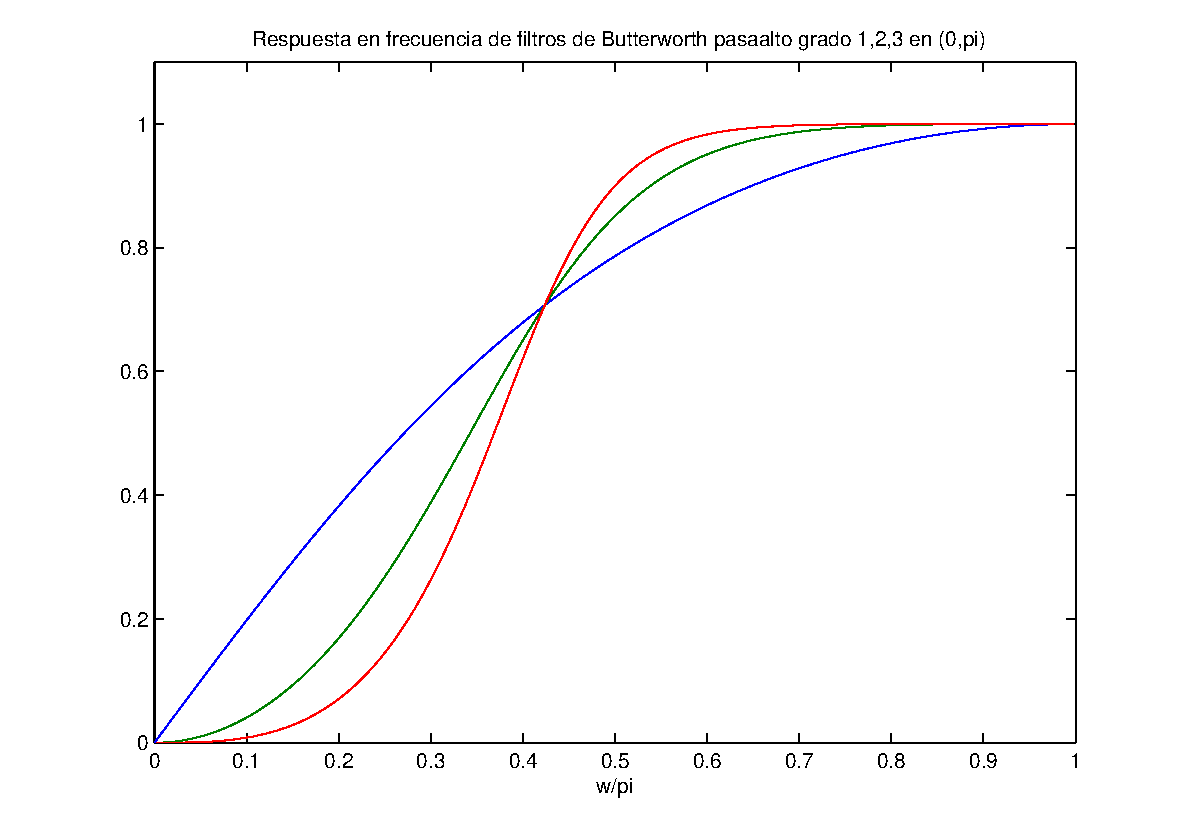
\includegraphics[width=14cm]{img/ej2}
%
\end{document}

Acá escribo cualquier mierda que se me cante y no sale nada!!!!!!!!!!!!!!
Como LaTeX encontró \end{document} ni se molesta en seguir procesando lo que sigue.
